\chapter{BroodwarBotQ}%: putting it all together}
%%% There's no difference between a pessimist who says, "Oh it's hopeless, so don’t bother doing anything." and an optimist who says, "Don't bother doing anything, it's going to turn out fine anyways. Either way, nothing happens.
%%% --Yvon Chouinard
\label{chapter:bot}


%%% BBQ LOC
%%% cpp:          23234

\begin{quotation}
\textit{Dealing with failure is easy: Work hard to improve. Success is also easy to handled: You've solved the wrong problem. Work hard to improve.}\\
\begin{flushright}Alan J. Perlis (1982)\end{flushright}
\end{quotation}

\lettrine{I}{n} this chapter, we present some of the engineering that went in the robotic player's (bot) implementation. We will also present the different flows of informations and how decisions are made during a game. Finally we will present the results of the full robotic player to various bots competitions.

\ifthenelse{\equal{\myebookformat}{false}}{
\chaptertoc
}{}



\citep{Wolfe11} % BOUNDED INTENTION PLANNING

\section{Code Architecture}

\label{sec:codearchitecture}
mapping schéma code <-> schéma info-flow.

\begin{figure}[h]
\begin{center}
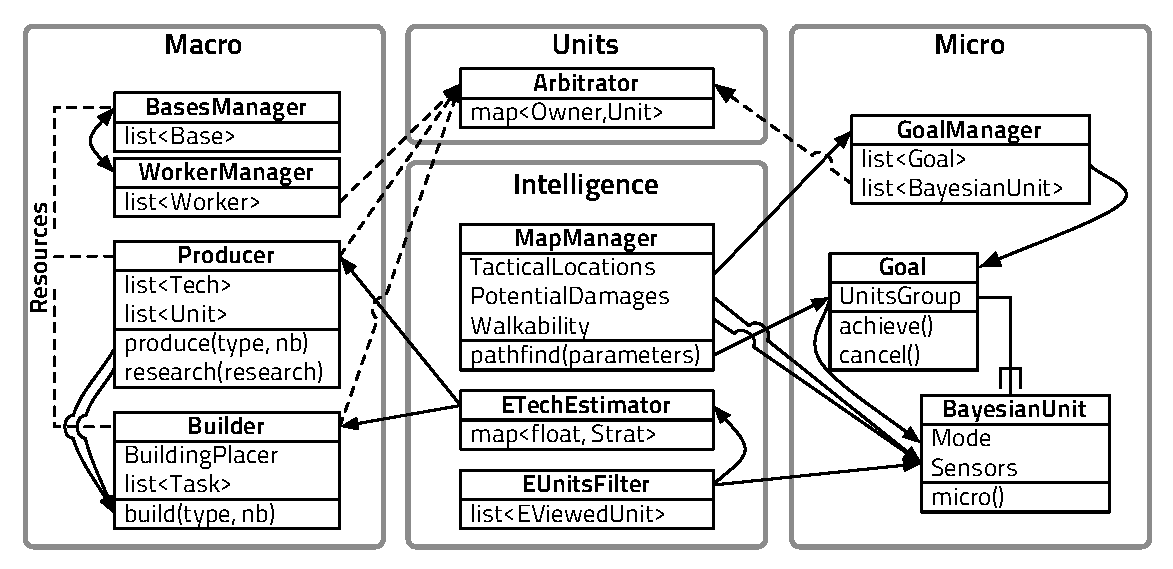
\includegraphics[width=16cm]{images/BBQEarly2012.pdf}
\caption{Simple view of the code architecture of \textsc{BroodwarBotQ}, the most important interactions are shown: every piece which has responsibility for the control of units refer to the \texttt{Arbitrator}, all macro components compete for resources, all other arrows represent orders or important transfers of information.}
\label{fig:codearchitecture}
\end{center}
\end{figure}

\subsection{Tactical Goals}
\label{sec:goals}
The decision that we want our AI system to make at this level is \textit{where} and \textit{how} to attack. This is reflected in the StarCraft bot as a \texttt{Goal} creation. \texttt{Goals} are interfacing high level tactical thinking with the steps necessary to their realization. A \texttt{Goal} recruits units and binds them under a \texttt{UnitsGroup} (see section~\ref{sec:unitsgroup}). A \texttt{Goal} is an \glos{FSM} in which two states are simple planners (an FSM with some form of procedural autonomy), it has:
\begin{itemize}
    \item preconditions, for instance a \textit{drop} attack needs to specify at least a transport unit (Shuttle/Dropship/Overlord) and ground attack units.
    \item hard states: \textit{waiting precondition, in progress, in cancel, achieved, canceled}, which corresponds to the \texttt{Goal} advancement..
    \item \textit{and} and/or \textit{or} logic subgoals with:
        \begin{itemize}
            \item a realization test
            \item a proposition of action to try to realize it
            \item an estimation of the ``distance'' to realization
        \end{itemize}
\end{itemize}
In the \textit{in progress} and \textit{in cancel} modes, the ``plan'' is a simple search in the achievable subgoals and their ``distance'' to realization.

The tactical model can specify \textit{where} to attack by setting a localized subgoal (Formation/See/Regroup/KillSubgoal...) to the right place. It can specify \textit{how} by setting the adequate precondition(s).


\section{A Game Walkthrough}
The tree of decisions.


\section{Results}

%%% AIIDE 2011
%%% Skynet
%%% UAlbertaBot
%%% Aiur
%%% ItayUndermind
%%% EISBot
%%% SPAR
%%% Undermind
%%% Nova
%%% BroodwarBotQ
%%% BTHAI
%%% Cromulent
%%% bigbrother
%%% Quorum

%%% CIG
%%% Crashes Games Bot Wins
%%% 0 30 Skynet 26
%%% 0 30 UAlbertaBot 22
%%% 3 30 Xelnaga 11
%%% 2 30 BroodwarBotQ 1
%%% 10 entries                    


